\documentclass[11pt]{article}
\usepackage[textwidth=18.0cm, textheight=23.0cm, top=2.0cm]{geometry}
\usepackage{pst-all}
\usepackage{amssymb}
\usepackage{tikz}
\usepackage{underscore}\begin{document}
\pagestyle{empty}


ClassName: \underline{\textbf{Class_10.2bp-48}}
\par
BinSize: \underline{\textbf{100 × 100}}
\par
ReduceSize: \underline{\textbf{100 × 100}}
\par
TypeNum: \underline{\textbf{98}}
\par
Num: \underline{\textbf{100}}
\par
OutS: \underline{\textbf{160000}}
\par
InS: \underline{\textbf{150659}}
\par
Rate: \underline{\textbf{0.942}}
\par
UB: \underline{\textbf{16}}
\par
LB0: \underline{\textbf{16}}
\par
LB: \underline{\textbf{16}}
\par
LBWithCut: \underline{\textbf{16}}
\par
NodeCut: \underline{\textbf{0}}
\par
ExtendedNodeCnt: \underline{\textbf{1}}
\par
GenNodeCnt: \underline{\textbf{1}}
\par
PrimalNode: \underline{\textbf{0}}
\par
ColumnCount: \underline{\textbf{16}}
\par
TotalCutCount: \underline{\textbf{0}}
\par
RootCutCount: \underline{\textbf{0}}
\par
LPSolverCnt: \underline{\textbf{1}}
\par
PricingSolverCnt: \underline{\textbf{0}}
\par
BranchAndBoundNum: \underline{\textbf{1}}
\par
isOpt: \underline{\textbf{true}}
\par
TimeOnInitSolution: \underline{\textbf{1.040 s}}
\par
TimeOnPrimal: \underline{\textbf{0.000 s}}
\par
TimeOnPricing: \underline{\textbf{0.000 s}}
\par
TimeOnRmp: \underline{\textbf{0.079 s}}
\par
TotalTime: \underline{\textbf{1.181 s}}
\par
\newpage


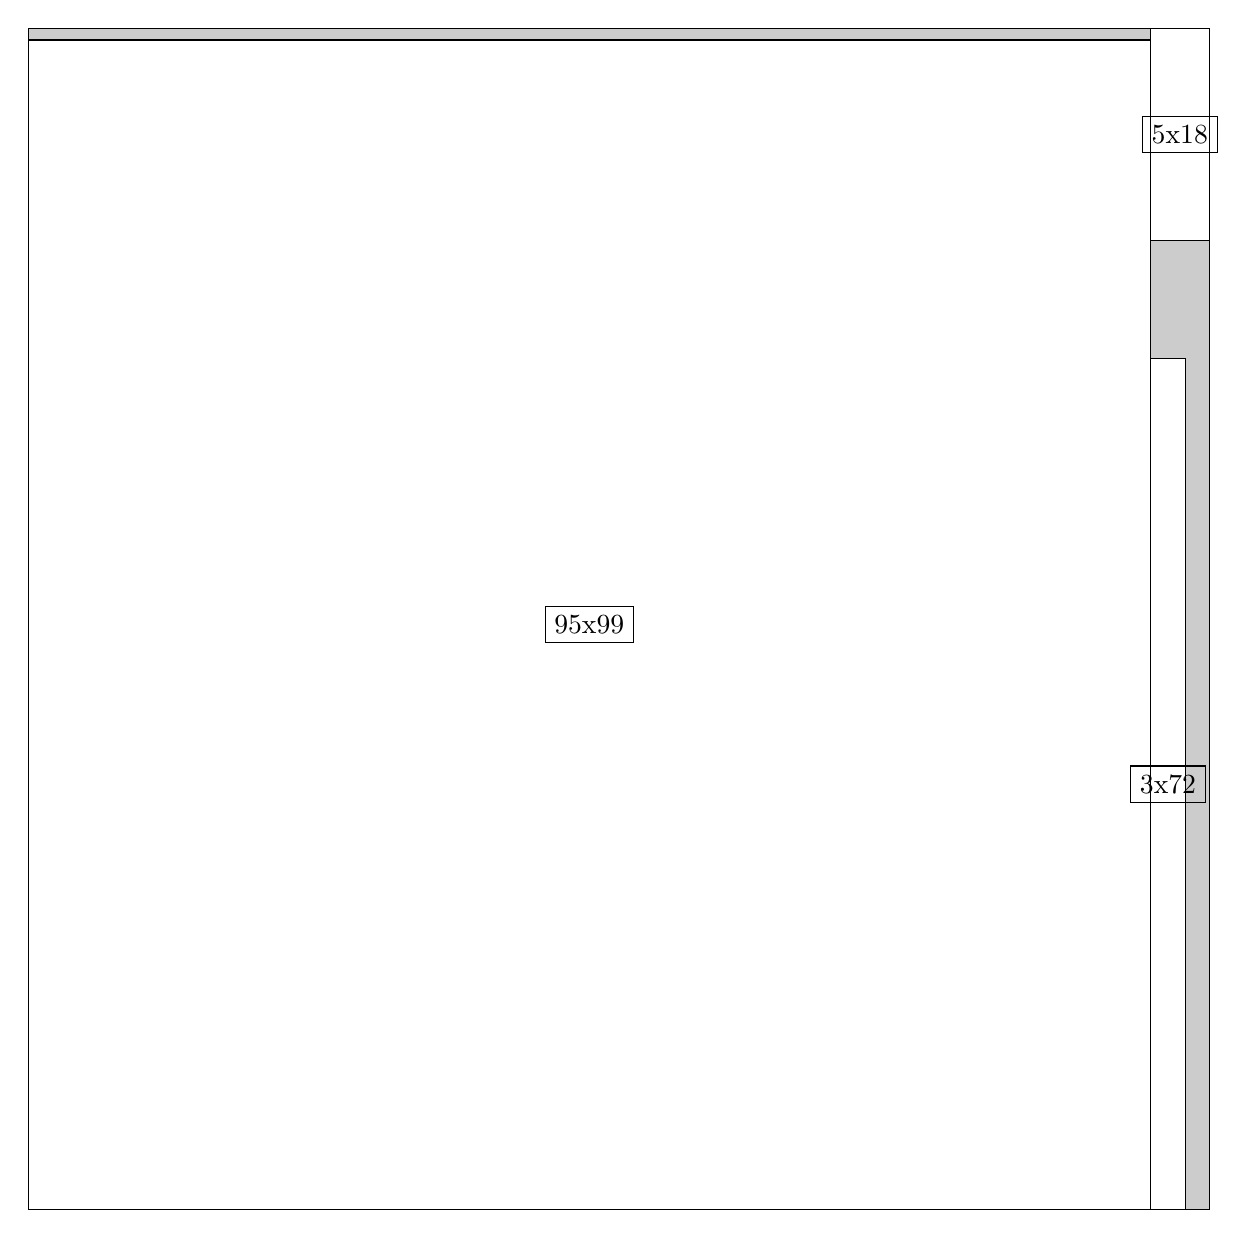
\begin{tikzpicture}[shorten >=1pt,scale=1.0,every node/.style={scale=1.0},->]
\tikzstyle{vertex}=[circle,fill=black!25,minimum size=14pt,inner sep=0pt]
\filldraw[fill=gray!40!white, draw=black] (0,0) rectangle (15.0,15.0);
\foreach \name/\x/\y/\w/\h in {95x99/0.0/0.0/14.25/14.85,3x72/14.25/0.0/0.44999999999999996/10.799999999999999,5x18/14.25/12.299999999999999/0.75/2.6999999999999997}
\filldraw[fill=white!40!white, draw=black] (\x,\y) rectangle node[draw] (\name) {\name} ++(\w,\h);
\end{tikzpicture}


w =95 , h =99 , x =0 , y =0 , v =9405
\par
w =3 , h =72 , x =95 , y =0 , v =216
\par
w =5 , h =18 , x =95 , y =82 , v =90
\par
\newpage


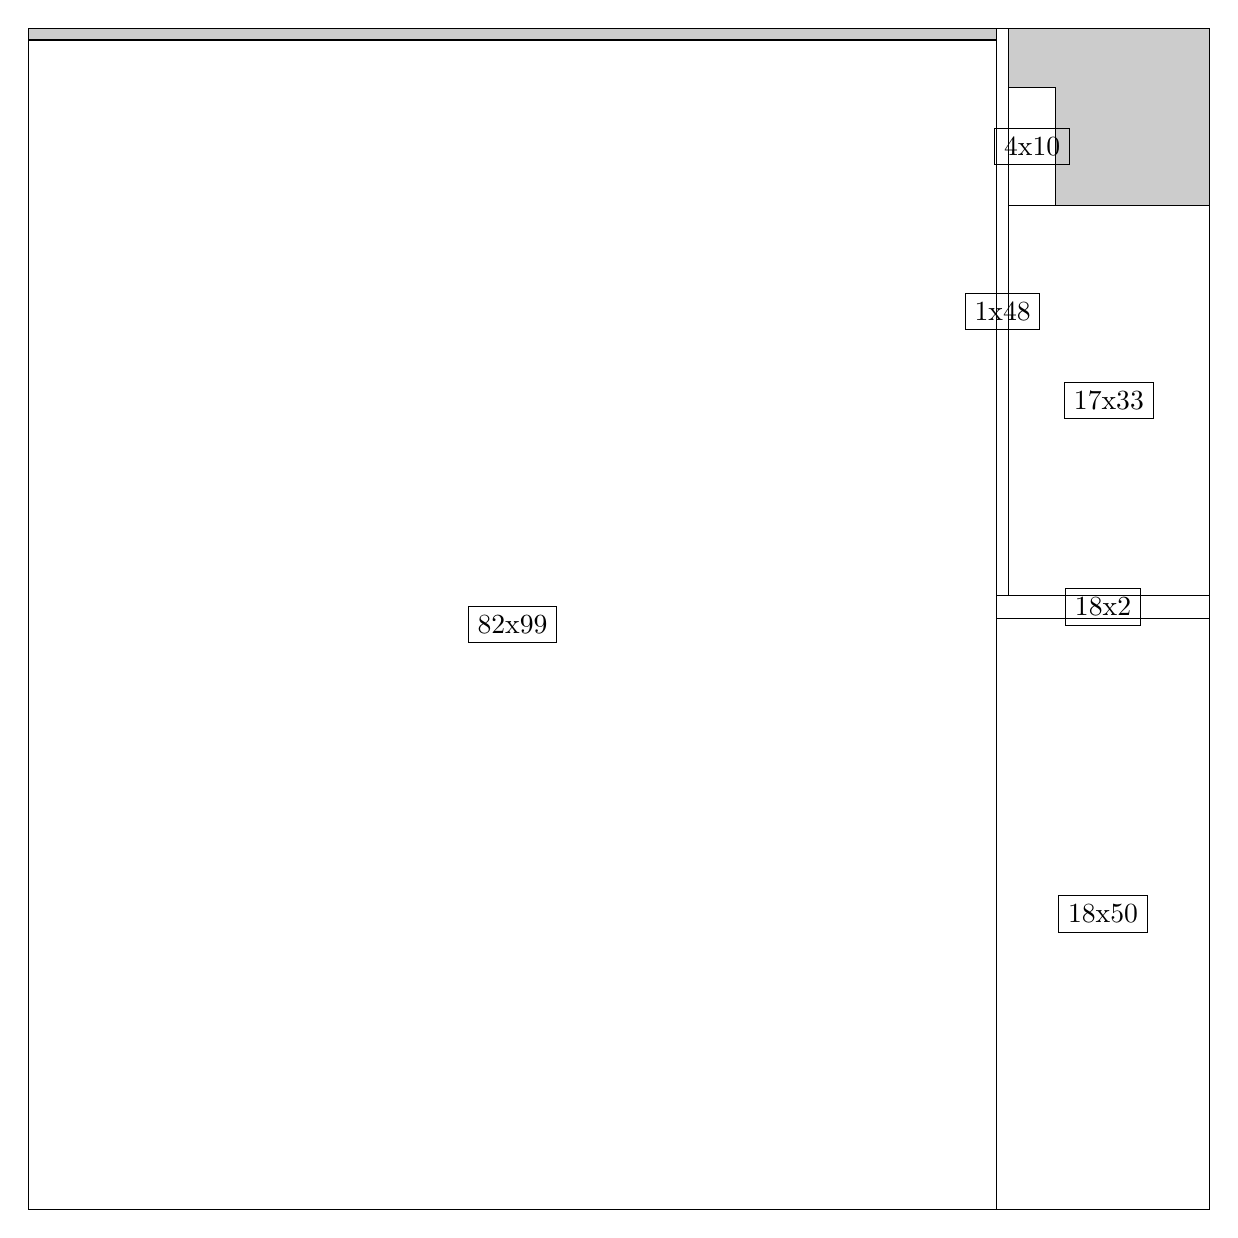
\begin{tikzpicture}[shorten >=1pt,scale=1.0,every node/.style={scale=1.0},->]
\tikzstyle{vertex}=[circle,fill=black!25,minimum size=14pt,inner sep=0pt]
\filldraw[fill=gray!40!white, draw=black] (0,0) rectangle (15.0,15.0);
\foreach \name/\x/\y/\w/\h in {82x99/0.0/0.0/12.299999999999999/14.85,18x50/12.299999999999999/0.0/2.6999999999999997/7.5,17x33/12.45/7.8/2.55/4.95,1x48/12.299999999999999/7.8/0.15/7.199999999999999,4x10/12.45/12.75/0.6/1.5,18x2/12.299999999999999/7.5/2.6999999999999997/0.3}
\filldraw[fill=white!40!white, draw=black] (\x,\y) rectangle node[draw] (\name) {\name} ++(\w,\h);
\end{tikzpicture}


w =82 , h =99 , x =0 , y =0 , v =8118
\par
w =18 , h =50 , x =82 , y =0 , v =900
\par
w =17 , h =33 , x =83 , y =52 , v =561
\par
w =1 , h =48 , x =82 , y =52 , v =48
\par
w =4 , h =10 , x =83 , y =85 , v =40
\par
w =18 , h =2 , x =82 , y =50 , v =36
\par
\newpage


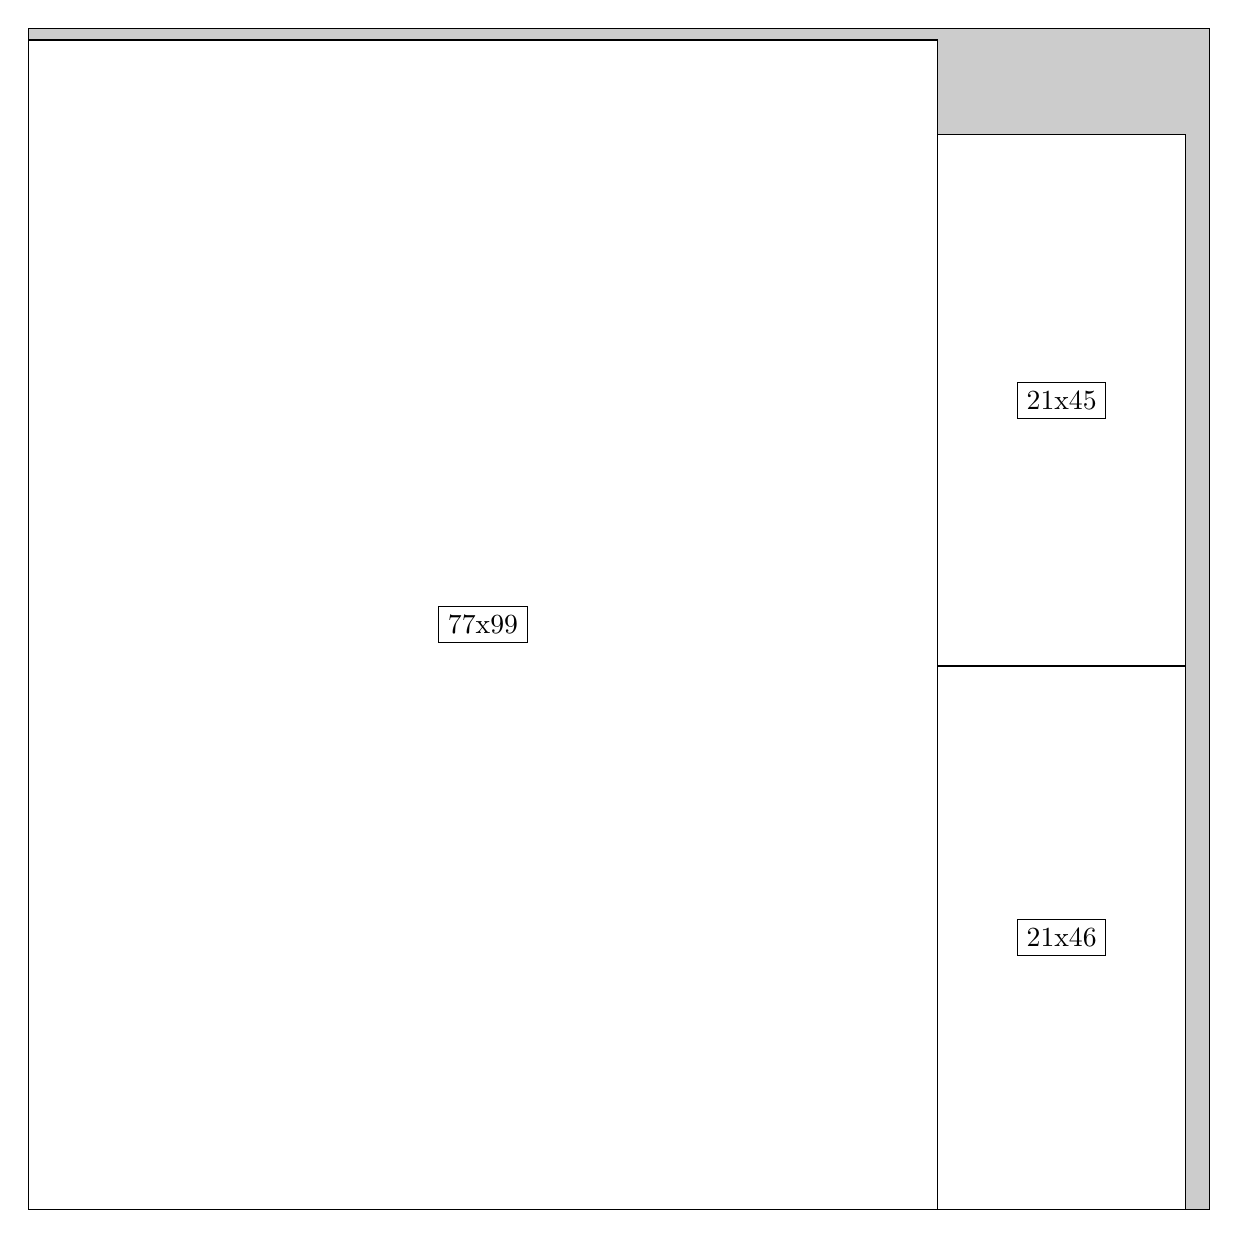
\begin{tikzpicture}[shorten >=1pt,scale=1.0,every node/.style={scale=1.0},->]
\tikzstyle{vertex}=[circle,fill=black!25,minimum size=14pt,inner sep=0pt]
\filldraw[fill=gray!40!white, draw=black] (0,0) rectangle (15.0,15.0);
\foreach \name/\x/\y/\w/\h in {77x99/0.0/0.0/11.549999999999999/14.85,21x46/11.549999999999999/0.0/3.15/6.8999999999999995,21x45/11.549999999999999/6.8999999999999995/3.15/6.75}
\filldraw[fill=white!40!white, draw=black] (\x,\y) rectangle node[draw] (\name) {\name} ++(\w,\h);
\end{tikzpicture}


w =77 , h =99 , x =0 , y =0 , v =7623
\par
w =21 , h =46 , x =77 , y =0 , v =966
\par
w =21 , h =45 , x =77 , y =46 , v =945
\par
\newpage


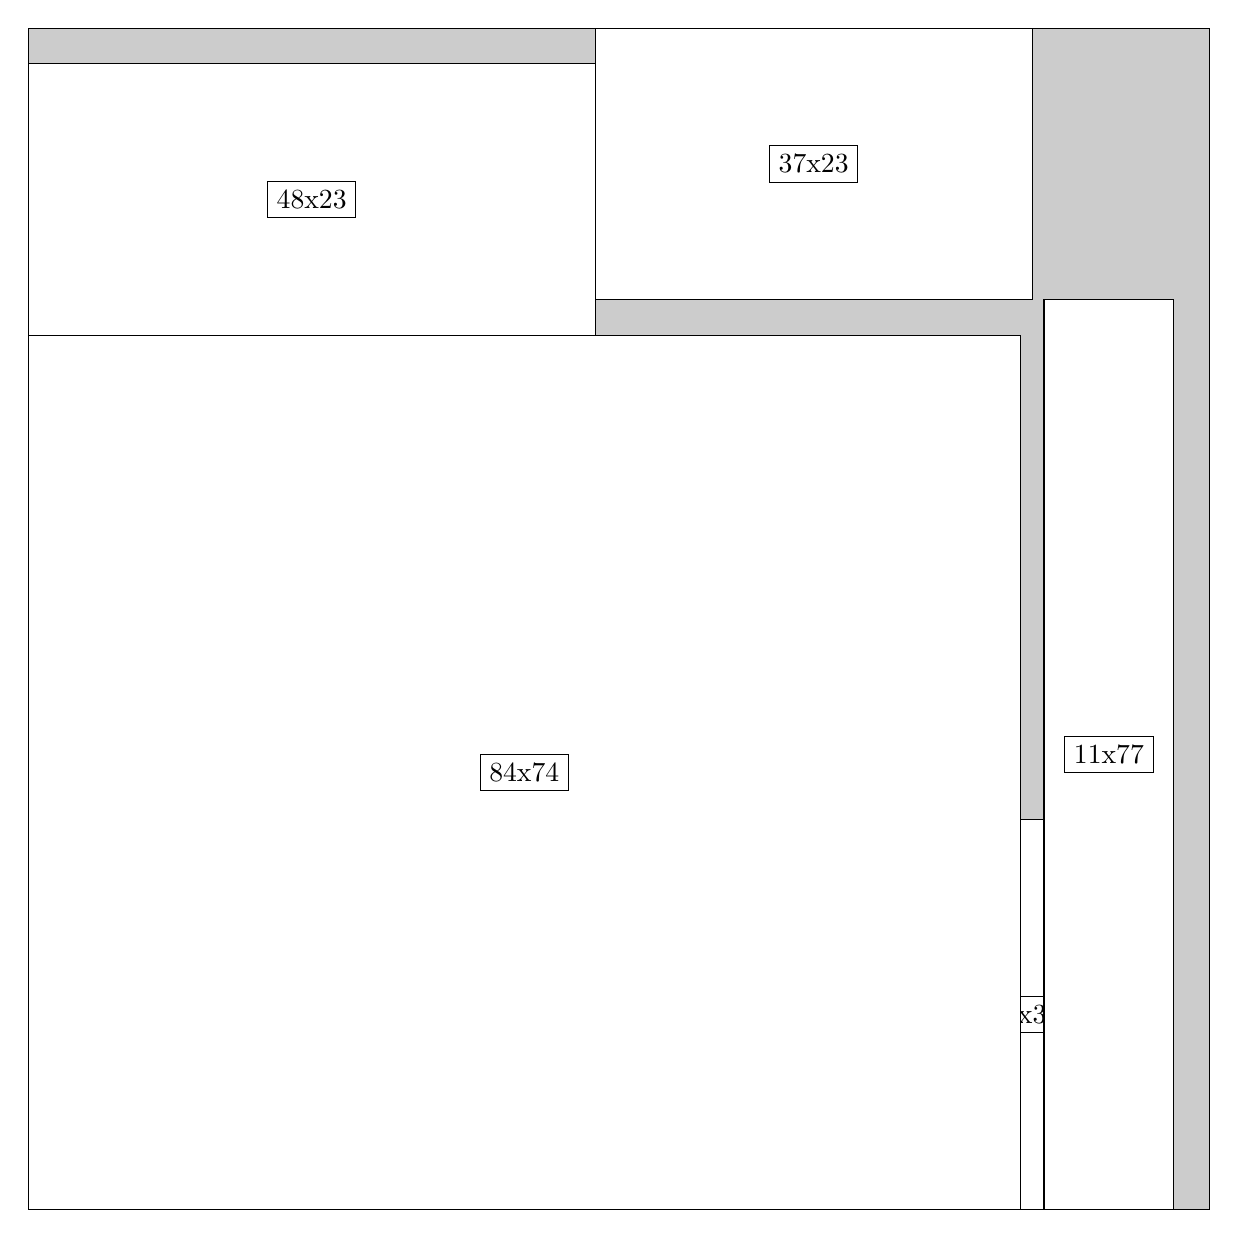
\begin{tikzpicture}[shorten >=1pt,scale=1.0,every node/.style={scale=1.0},->]
\tikzstyle{vertex}=[circle,fill=black!25,minimum size=14pt,inner sep=0pt]
\filldraw[fill=gray!40!white, draw=black] (0,0) rectangle (15.0,15.0);
\foreach \name/\x/\y/\w/\h in {2x33/12.6/0.0/0.3/4.95,48x23/0.0/11.1/7.199999999999999/3.4499999999999997,37x23/7.199999999999999/11.549999999999999/5.55/3.4499999999999997,11x77/12.9/0.0/1.65/11.549999999999999,84x74/0.0/0.0/12.6/11.1}
\filldraw[fill=white!40!white, draw=black] (\x,\y) rectangle node[draw] (\name) {\name} ++(\w,\h);
\end{tikzpicture}


w =2 , h =33 , x =84 , y =0 , v =66
\par
w =48 , h =23 , x =0 , y =74 , v =1104
\par
w =37 , h =23 , x =48 , y =77 , v =851
\par
w =11 , h =77 , x =86 , y =0 , v =847
\par
w =84 , h =74 , x =0 , y =0 , v =6216
\par
\newpage


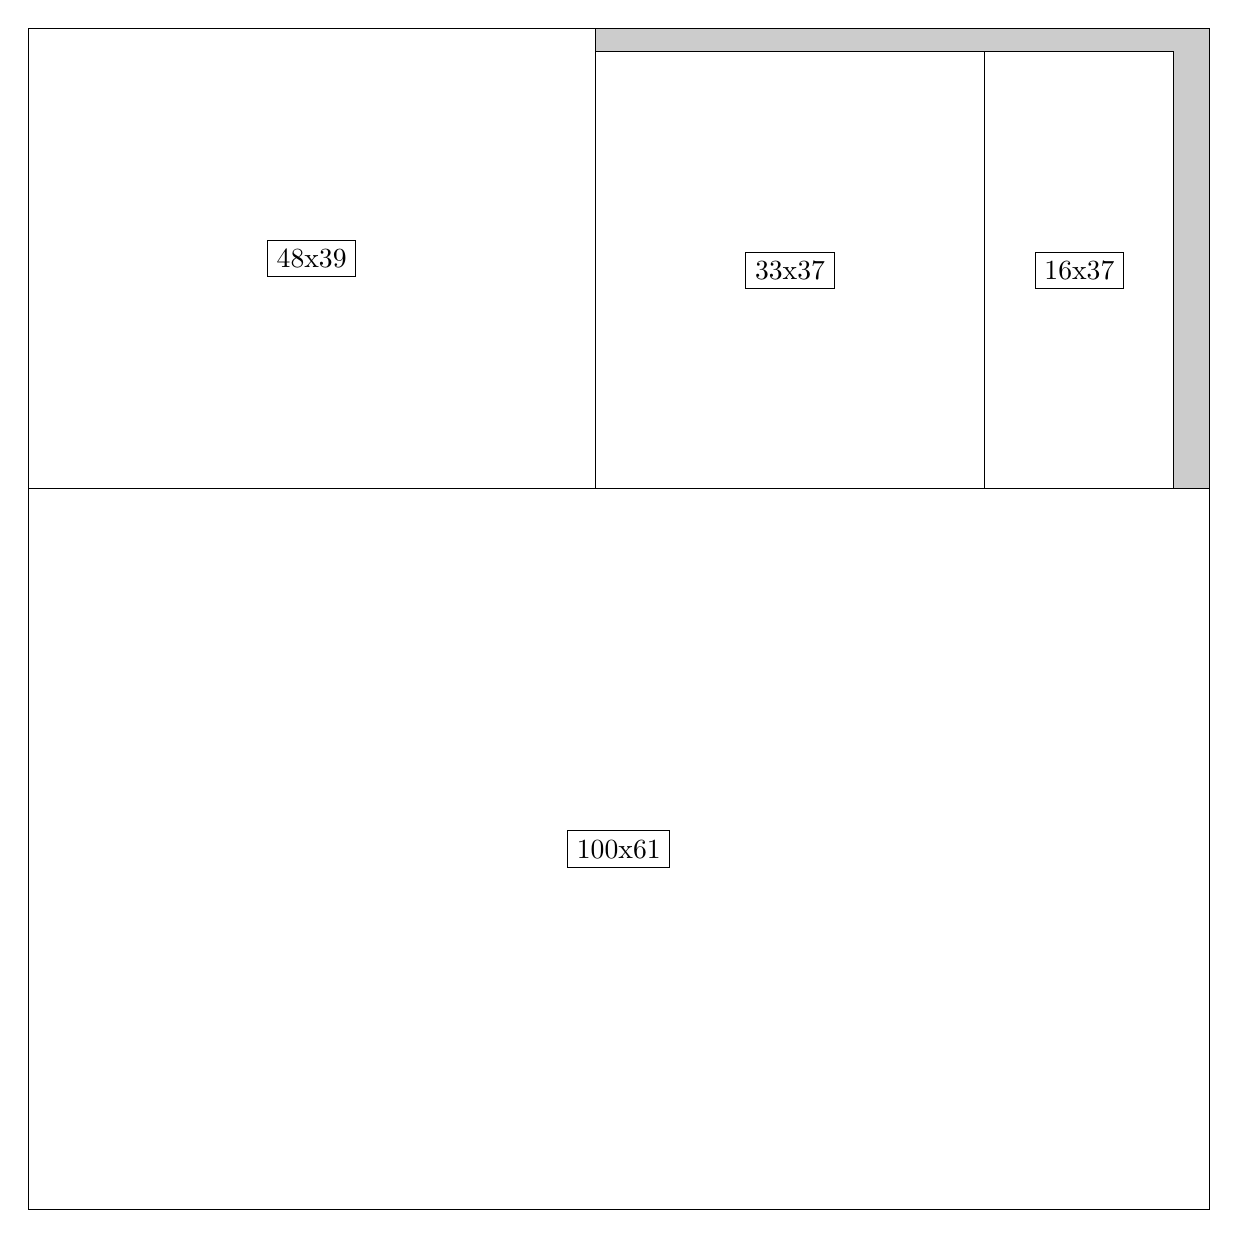
\begin{tikzpicture}[shorten >=1pt,scale=1.0,every node/.style={scale=1.0},->]
\tikzstyle{vertex}=[circle,fill=black!25,minimum size=14pt,inner sep=0pt]
\filldraw[fill=gray!40!white, draw=black] (0,0) rectangle (15.0,15.0);
\foreach \name/\x/\y/\w/\h in {100x61/0.0/0.0/15.0/9.15,48x39/0.0/9.15/7.199999999999999/5.85,33x37/7.199999999999999/9.15/4.95/5.55,16x37/12.15/9.15/2.4/5.55}
\filldraw[fill=white!40!white, draw=black] (\x,\y) rectangle node[draw] (\name) {\name} ++(\w,\h);
\end{tikzpicture}


w =100 , h =61 , x =0 , y =0 , v =6100
\par
w =48 , h =39 , x =0 , y =61 , v =1872
\par
w =33 , h =37 , x =48 , y =61 , v =1221
\par
w =16 , h =37 , x =81 , y =61 , v =592
\par
\newpage


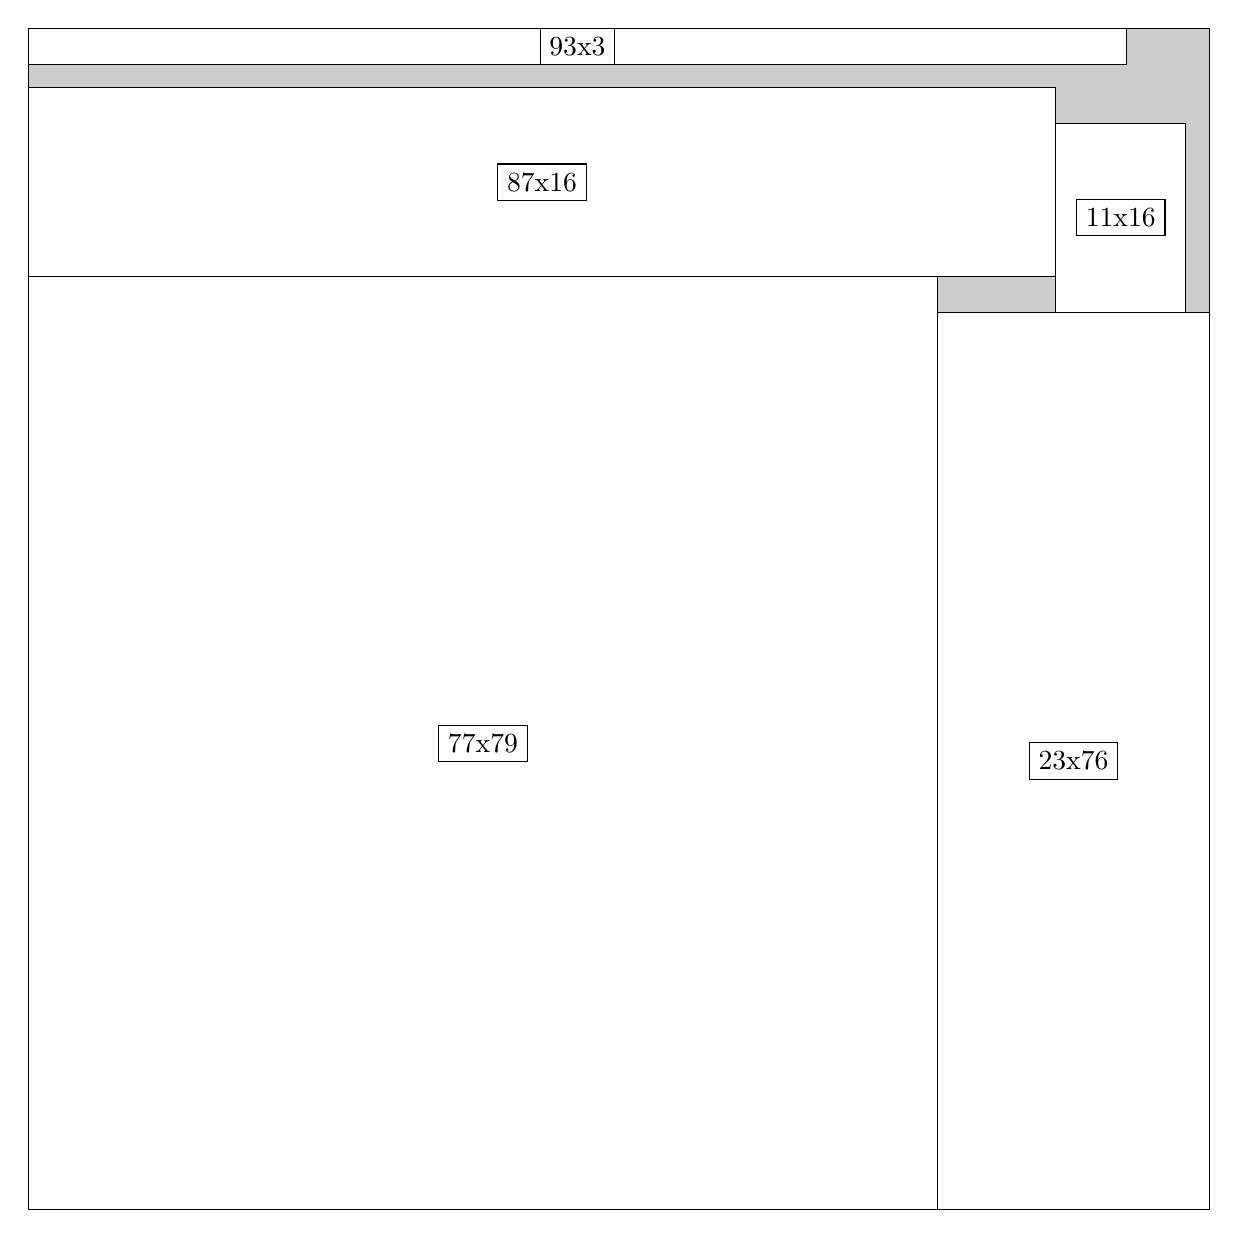
\begin{tikzpicture}[shorten >=1pt,scale=1.0,every node/.style={scale=1.0},->]
\tikzstyle{vertex}=[circle,fill=black!25,minimum size=14pt,inner sep=0pt]
\filldraw[fill=gray!40!white, draw=black] (0,0) rectangle (15.0,15.0);
\foreach \name/\x/\y/\w/\h in {77x79/0.0/0.0/11.549999999999999/11.85,23x76/11.549999999999999/0.0/3.4499999999999997/11.4,87x16/0.0/11.85/13.049999999999999/2.4,93x3/0.0/14.549999999999999/13.95/0.44999999999999996,11x16/13.049999999999999/11.4/1.65/2.4}
\filldraw[fill=white!40!white, draw=black] (\x,\y) rectangle node[draw] (\name) {\name} ++(\w,\h);
\end{tikzpicture}


w =77 , h =79 , x =0 , y =0 , v =6083
\par
w =23 , h =76 , x =77 , y =0 , v =1748
\par
w =87 , h =16 , x =0 , y =79 , v =1392
\par
w =93 , h =3 , x =0 , y =97 , v =279
\par
w =11 , h =16 , x =87 , y =76 , v =176
\par
\newpage


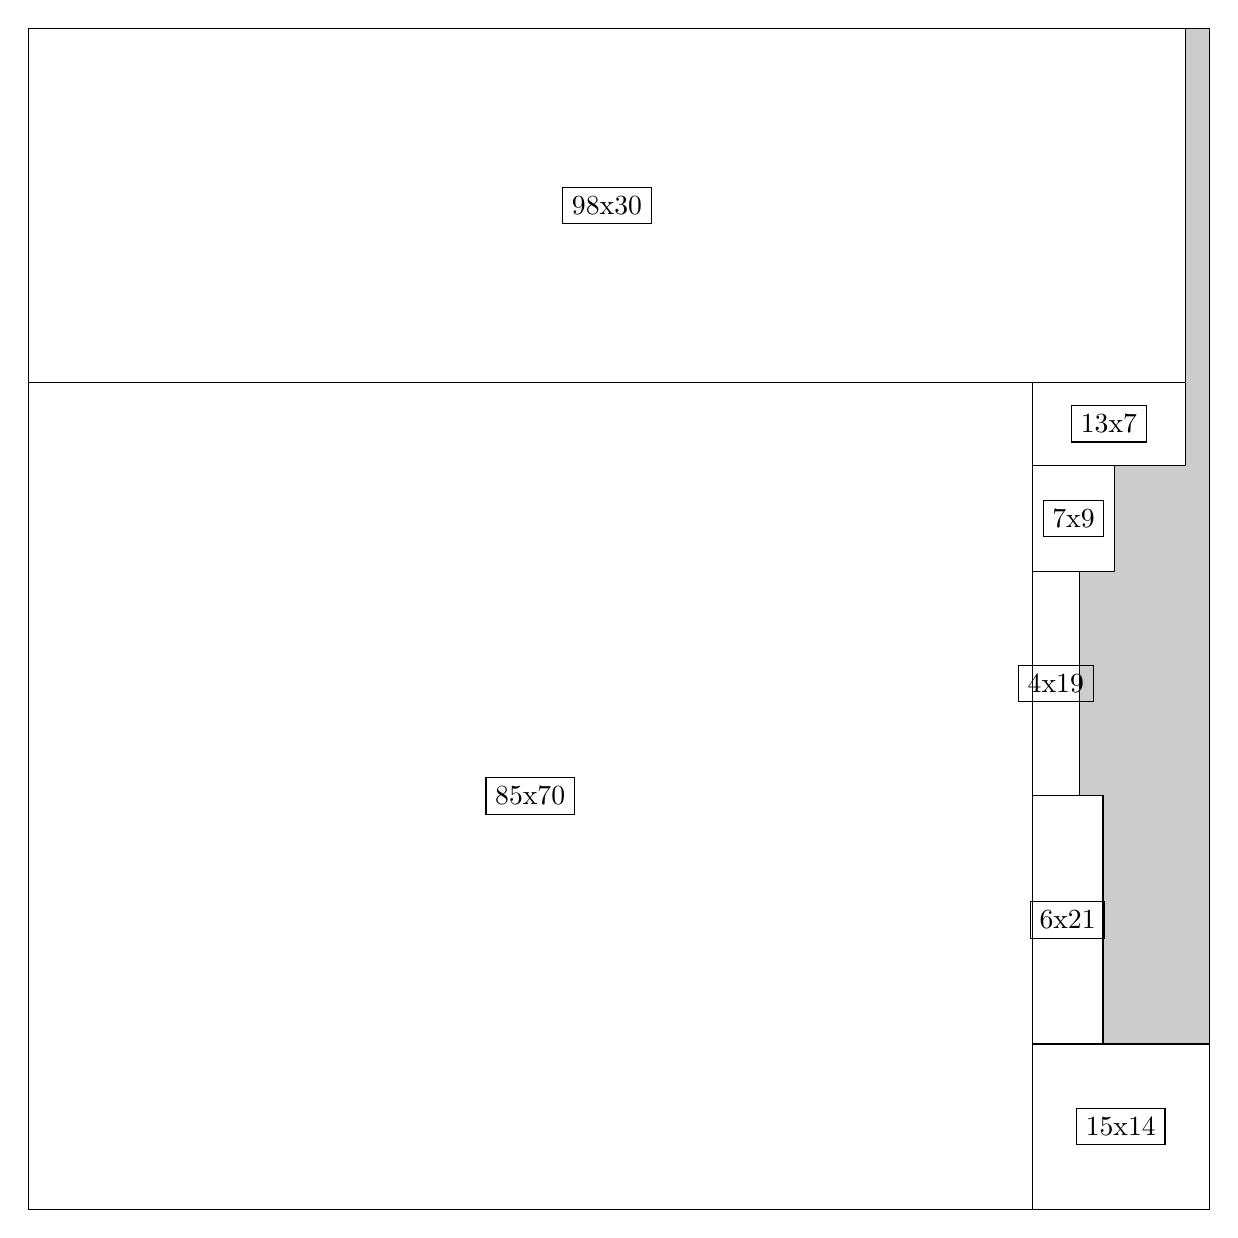
\begin{tikzpicture}[shorten >=1pt,scale=1.0,every node/.style={scale=1.0},->]
\tikzstyle{vertex}=[circle,fill=black!25,minimum size=14pt,inner sep=0pt]
\filldraw[fill=gray!40!white, draw=black] (0,0) rectangle (15.0,15.0);
\foreach \name/\x/\y/\w/\h in {85x70/0.0/0.0/12.75/10.5,98x30/0.0/10.5/14.7/4.5,15x14/12.75/0.0/2.25/2.1,6x21/12.75/2.1/0.8999999999999999/3.15,13x7/12.75/9.45/1.95/1.05,4x19/12.75/5.25/0.6/2.85,7x9/12.75/8.1/1.05/1.3499999999999999}
\filldraw[fill=white!40!white, draw=black] (\x,\y) rectangle node[draw] (\name) {\name} ++(\w,\h);
\end{tikzpicture}


w =85 , h =70 , x =0 , y =0 , v =5950
\par
w =98 , h =30 , x =0 , y =70 , v =2940
\par
w =15 , h =14 , x =85 , y =0 , v =210
\par
w =6 , h =21 , x =85 , y =14 , v =126
\par
w =13 , h =7 , x =85 , y =63 , v =91
\par
w =4 , h =19 , x =85 , y =35 , v =76
\par
w =7 , h =9 , x =85 , y =54 , v =63
\par
\newpage


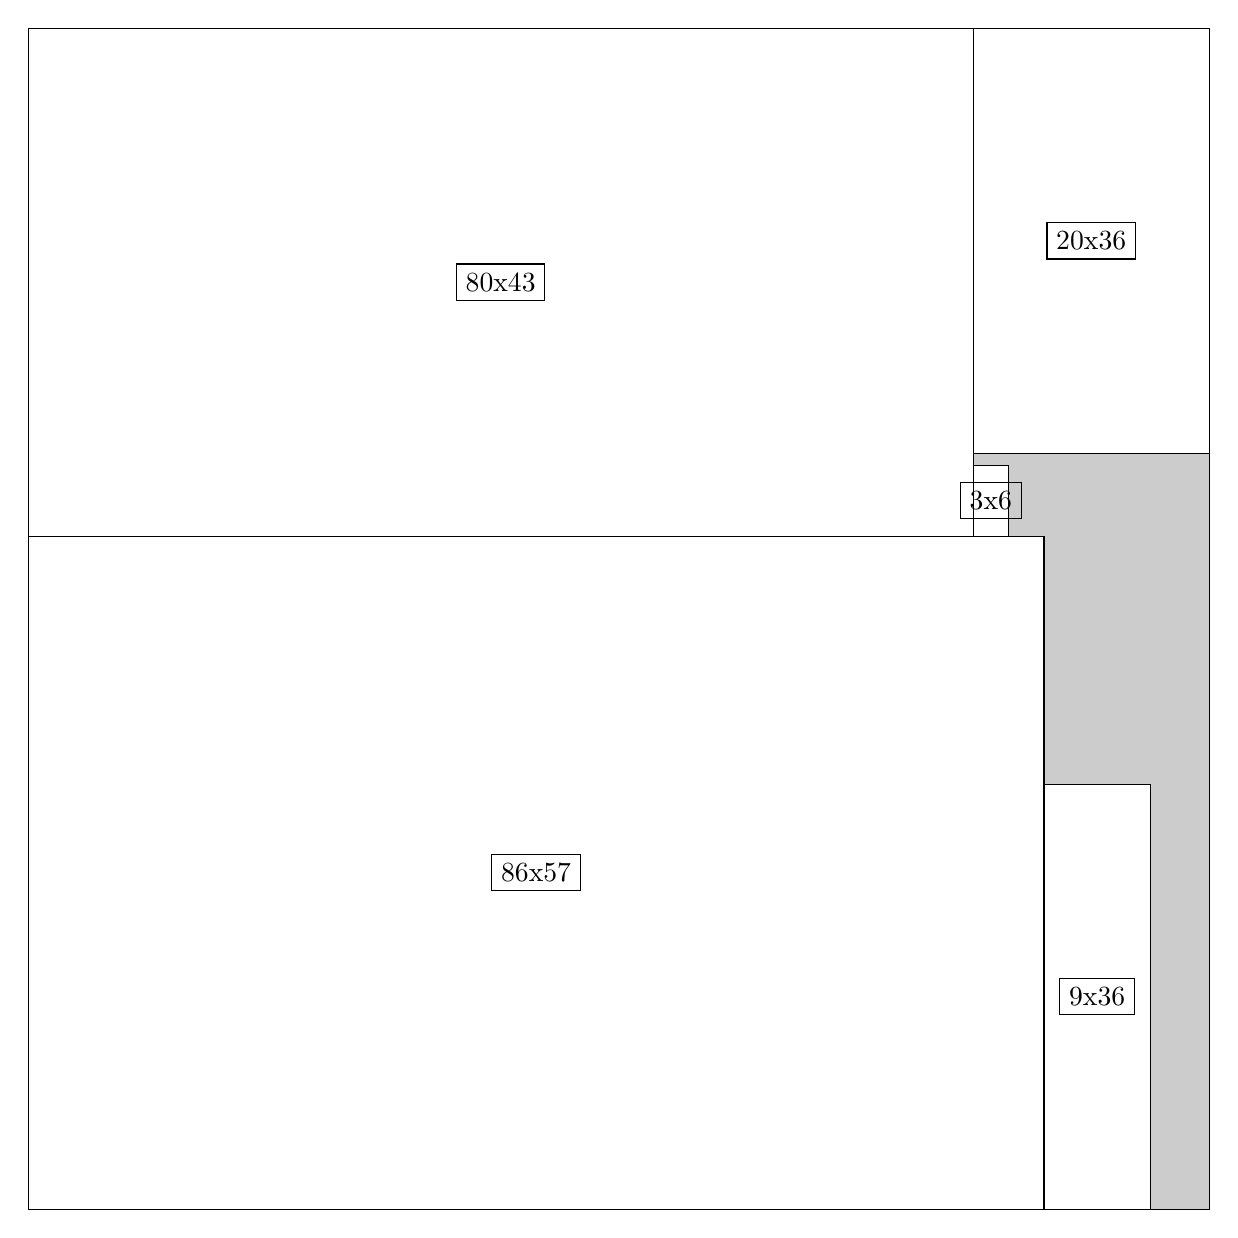
\begin{tikzpicture}[shorten >=1pt,scale=1.0,every node/.style={scale=1.0},->]
\tikzstyle{vertex}=[circle,fill=black!25,minimum size=14pt,inner sep=0pt]
\filldraw[fill=gray!40!white, draw=black] (0,0) rectangle (15.0,15.0);
\foreach \name/\x/\y/\w/\h in {86x57/0.0/0.0/12.9/8.549999999999999,80x43/0.0/8.549999999999999/12.0/6.45,20x36/12.0/9.6/3.0/5.3999999999999995,9x36/12.9/0.0/1.3499999999999999/5.3999999999999995,3x6/12.0/8.549999999999999/0.44999999999999996/0.8999999999999999}
\filldraw[fill=white!40!white, draw=black] (\x,\y) rectangle node[draw] (\name) {\name} ++(\w,\h);
\end{tikzpicture}


w =86 , h =57 , x =0 , y =0 , v =4902
\par
w =80 , h =43 , x =0 , y =57 , v =3440
\par
w =20 , h =36 , x =80 , y =64 , v =720
\par
w =9 , h =36 , x =86 , y =0 , v =324
\par
w =3 , h =6 , x =80 , y =57 , v =18
\par
\newpage


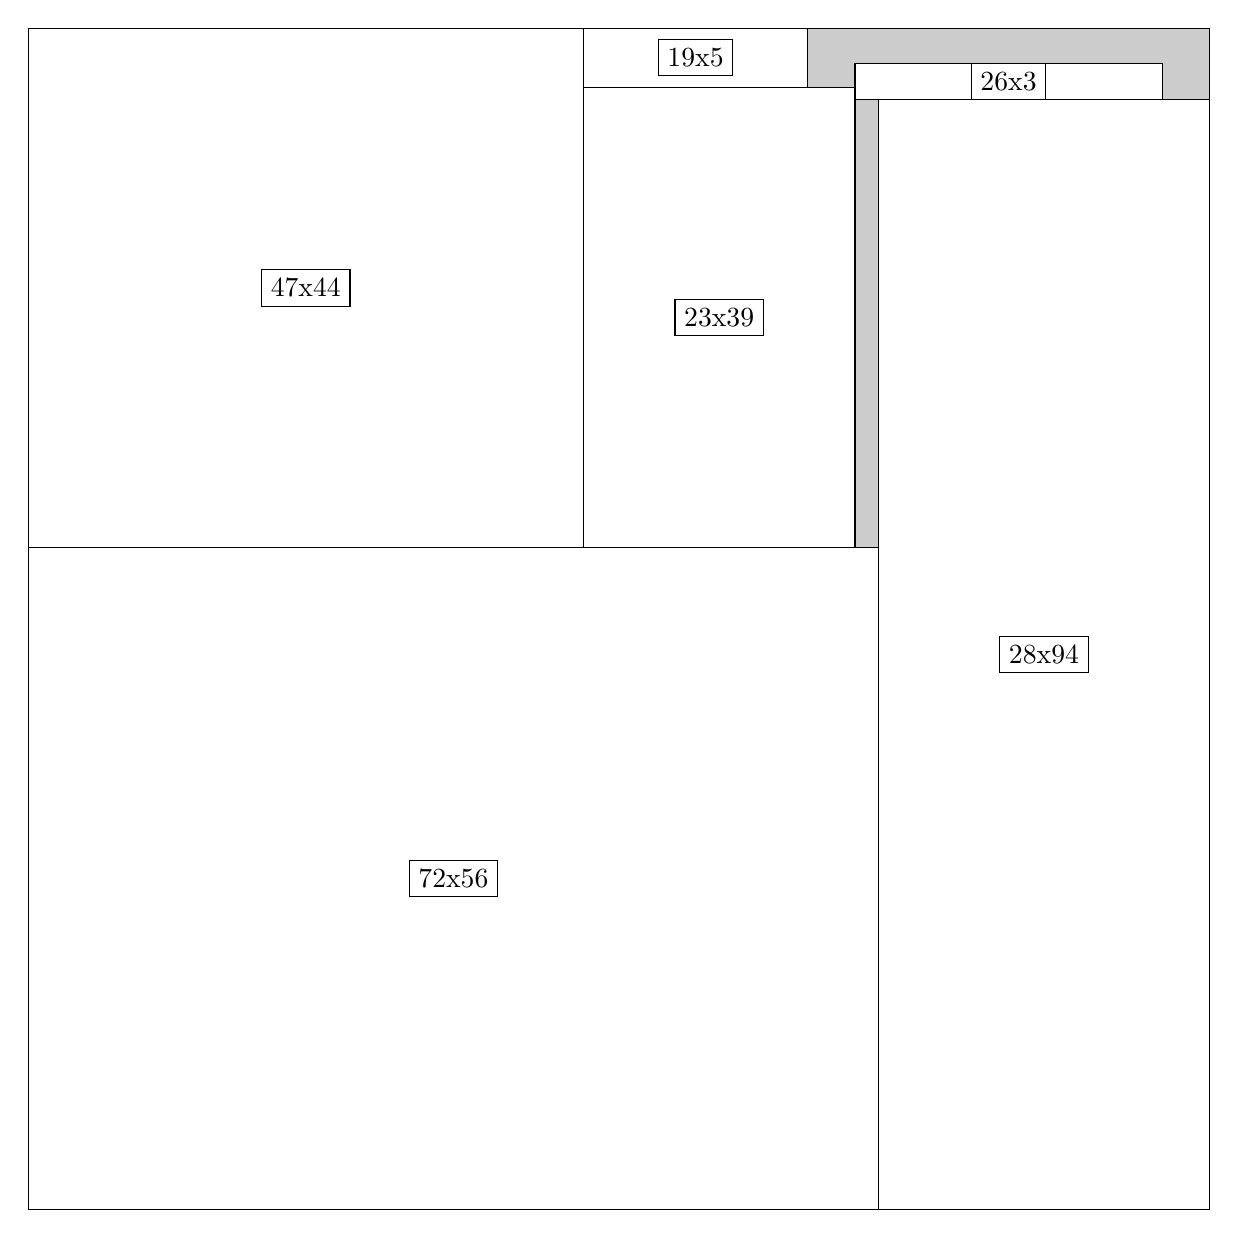
\begin{tikzpicture}[shorten >=1pt,scale=1.0,every node/.style={scale=1.0},->]
\tikzstyle{vertex}=[circle,fill=black!25,minimum size=14pt,inner sep=0pt]
\filldraw[fill=gray!40!white, draw=black] (0,0) rectangle (15.0,15.0);
\foreach \name/\x/\y/\w/\h in {72x56/0.0/0.0/10.799999999999999/8.4,28x94/10.799999999999999/0.0/4.2/14.1,47x44/0.0/8.4/7.05/6.6,23x39/7.05/8.4/3.4499999999999997/5.85,19x5/7.05/14.25/2.85/0.75,26x3/10.5/14.1/3.9/0.44999999999999996}
\filldraw[fill=white!40!white, draw=black] (\x,\y) rectangle node[draw] (\name) {\name} ++(\w,\h);
\end{tikzpicture}


w =72 , h =56 , x =0 , y =0 , v =4032
\par
w =28 , h =94 , x =72 , y =0 , v =2632
\par
w =47 , h =44 , x =0 , y =56 , v =2068
\par
w =23 , h =39 , x =47 , y =56 , v =897
\par
w =19 , h =5 , x =47 , y =95 , v =95
\par
w =26 , h =3 , x =70 , y =94 , v =78
\par
\newpage


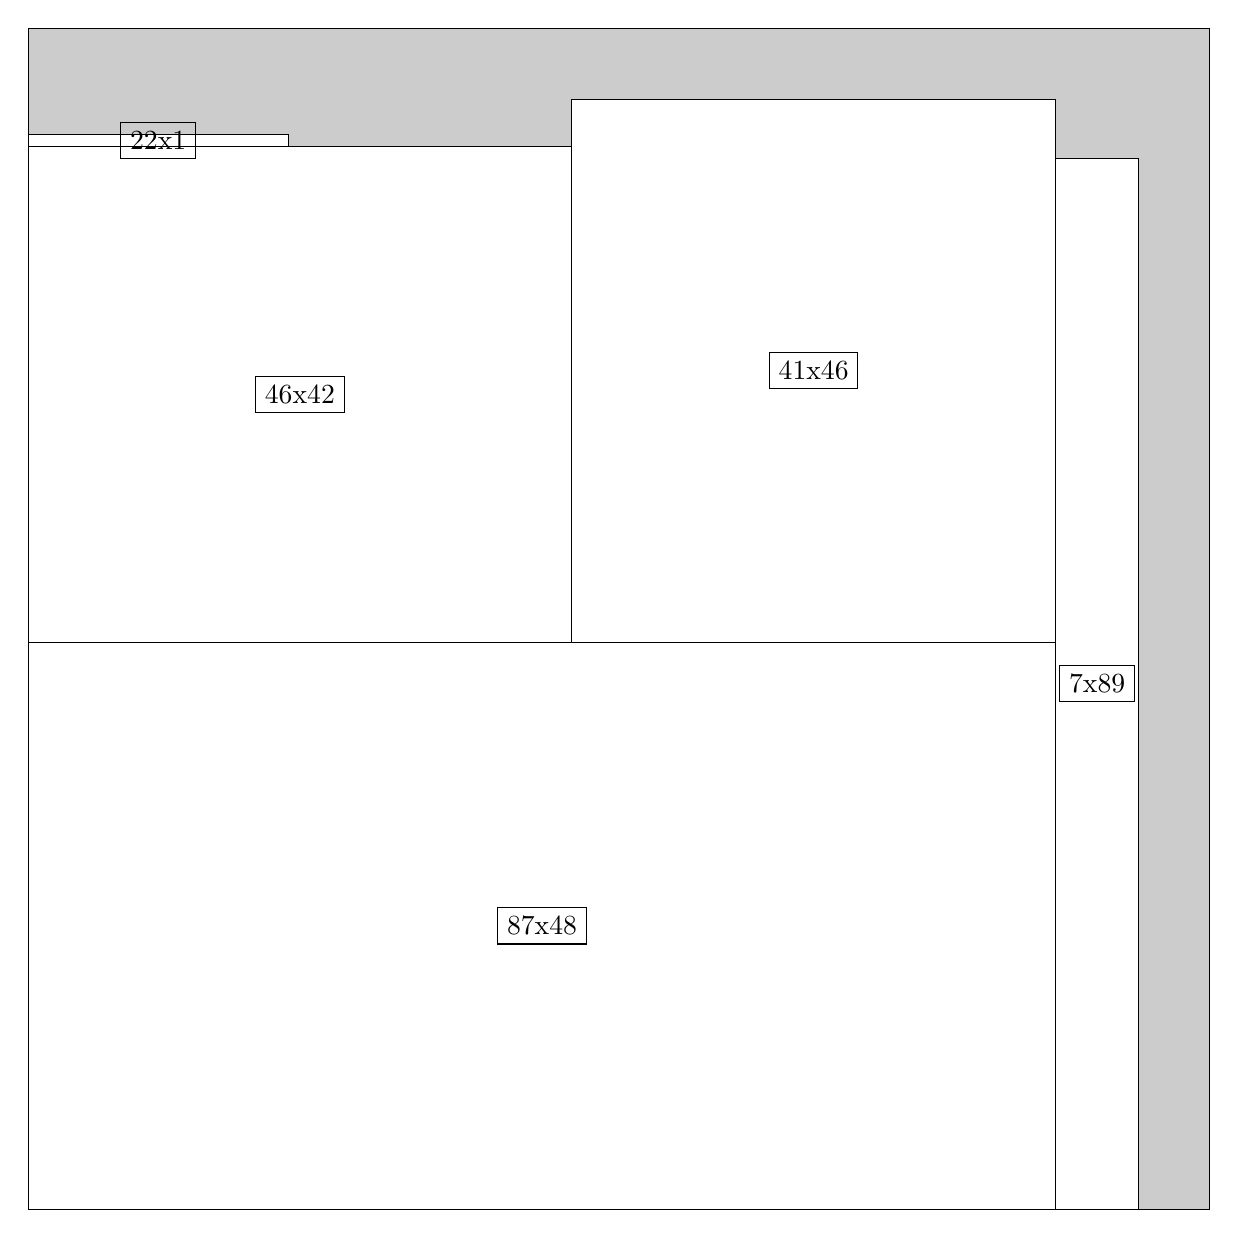
\begin{tikzpicture}[shorten >=1pt,scale=1.0,every node/.style={scale=1.0},->]
\tikzstyle{vertex}=[circle,fill=black!25,minimum size=14pt,inner sep=0pt]
\filldraw[fill=gray!40!white, draw=black] (0,0) rectangle (15.0,15.0);
\foreach \name/\x/\y/\w/\h in {87x48/0.0/0.0/13.049999999999999/7.199999999999999,46x42/0.0/7.199999999999999/6.8999999999999995/6.3,41x46/6.8999999999999995/7.199999999999999/6.1499999999999995/6.8999999999999995,7x89/13.049999999999999/0.0/1.05/13.35,22x1/0.0/13.5/3.3/0.15}
\filldraw[fill=white!40!white, draw=black] (\x,\y) rectangle node[draw] (\name) {\name} ++(\w,\h);
\end{tikzpicture}


w =87 , h =48 , x =0 , y =0 , v =4176
\par
w =46 , h =42 , x =0 , y =48 , v =1932
\par
w =41 , h =46 , x =46 , y =48 , v =1886
\par
w =7 , h =89 , x =87 , y =0 , v =623
\par
w =22 , h =1 , x =0 , y =90 , v =22
\par
\newpage


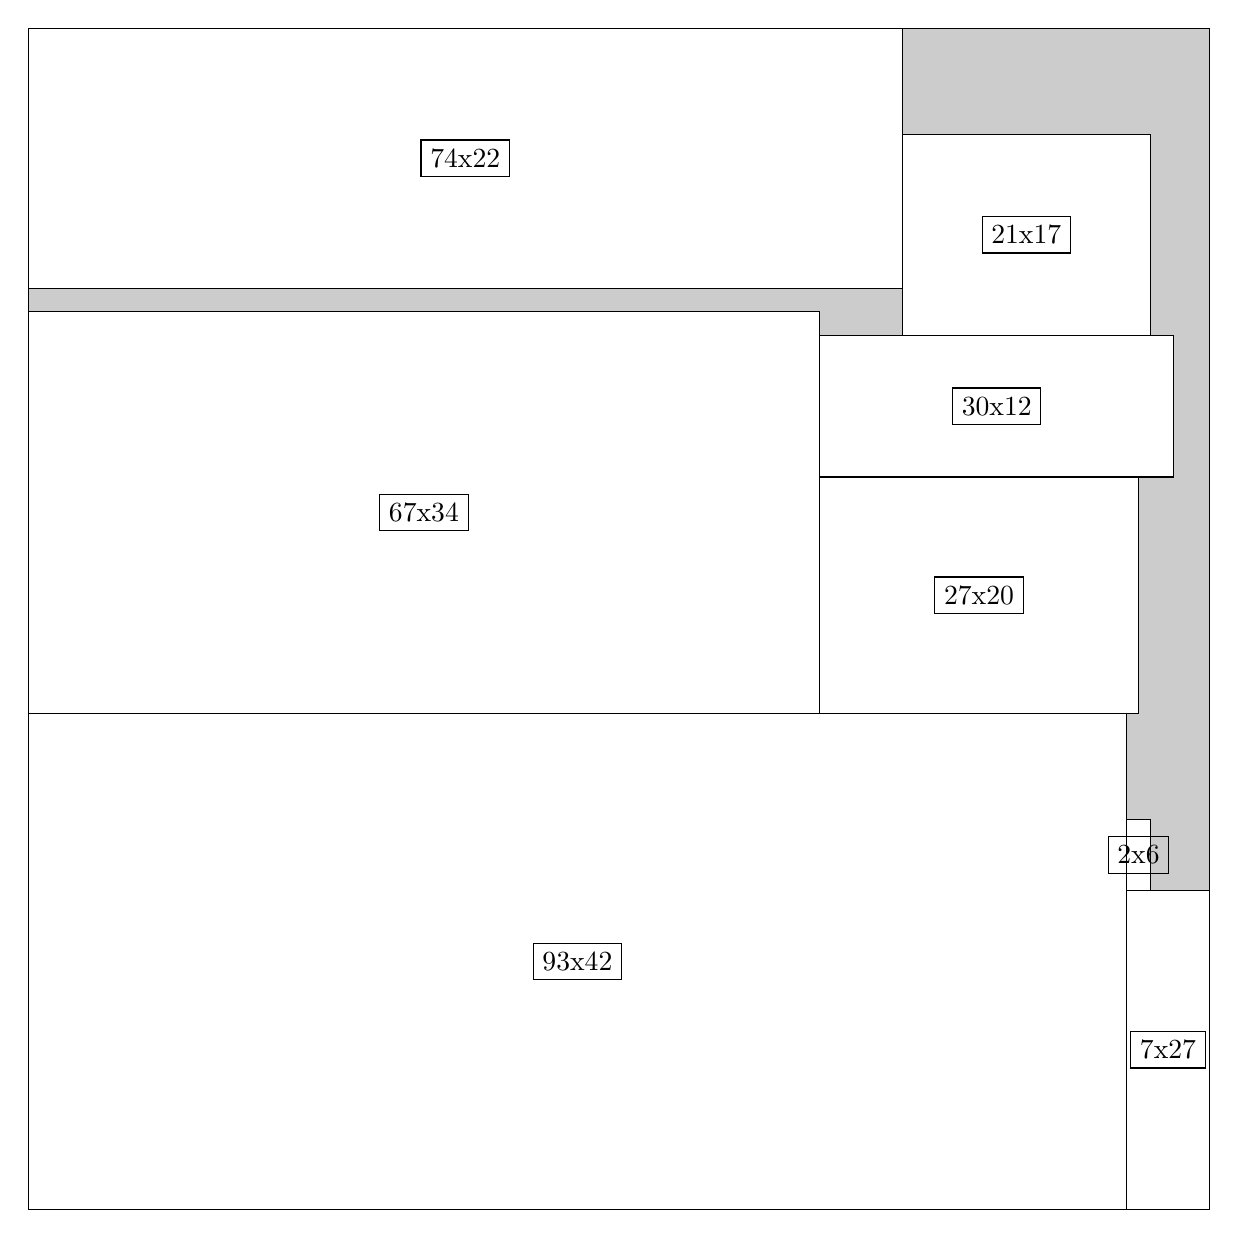
\begin{tikzpicture}[shorten >=1pt,scale=1.0,every node/.style={scale=1.0},->]
\tikzstyle{vertex}=[circle,fill=black!25,minimum size=14pt,inner sep=0pt]
\filldraw[fill=gray!40!white, draw=black] (0,0) rectangle (15.0,15.0);
\foreach \name/\x/\y/\w/\h in {93x42/0.0/0.0/13.95/6.3,67x34/0.0/6.3/10.049999999999999/5.1,74x22/0.0/11.7/11.1/3.3,27x20/10.049999999999999/6.3/4.05/3.0,30x12/10.049999999999999/9.299999999999999/4.5/1.7999999999999998,21x17/11.1/11.1/3.15/2.55,7x27/13.95/0.0/1.05/4.05,2x6/13.95/4.05/0.3/0.8999999999999999}
\filldraw[fill=white!40!white, draw=black] (\x,\y) rectangle node[draw] (\name) {\name} ++(\w,\h);
\end{tikzpicture}


w =93 , h =42 , x =0 , y =0 , v =3906
\par
w =67 , h =34 , x =0 , y =42 , v =2278
\par
w =74 , h =22 , x =0 , y =78 , v =1628
\par
w =27 , h =20 , x =67 , y =42 , v =540
\par
w =30 , h =12 , x =67 , y =62 , v =360
\par
w =21 , h =17 , x =74 , y =74 , v =357
\par
w =7 , h =27 , x =93 , y =0 , v =189
\par
w =2 , h =6 , x =93 , y =27 , v =12
\par
\newpage


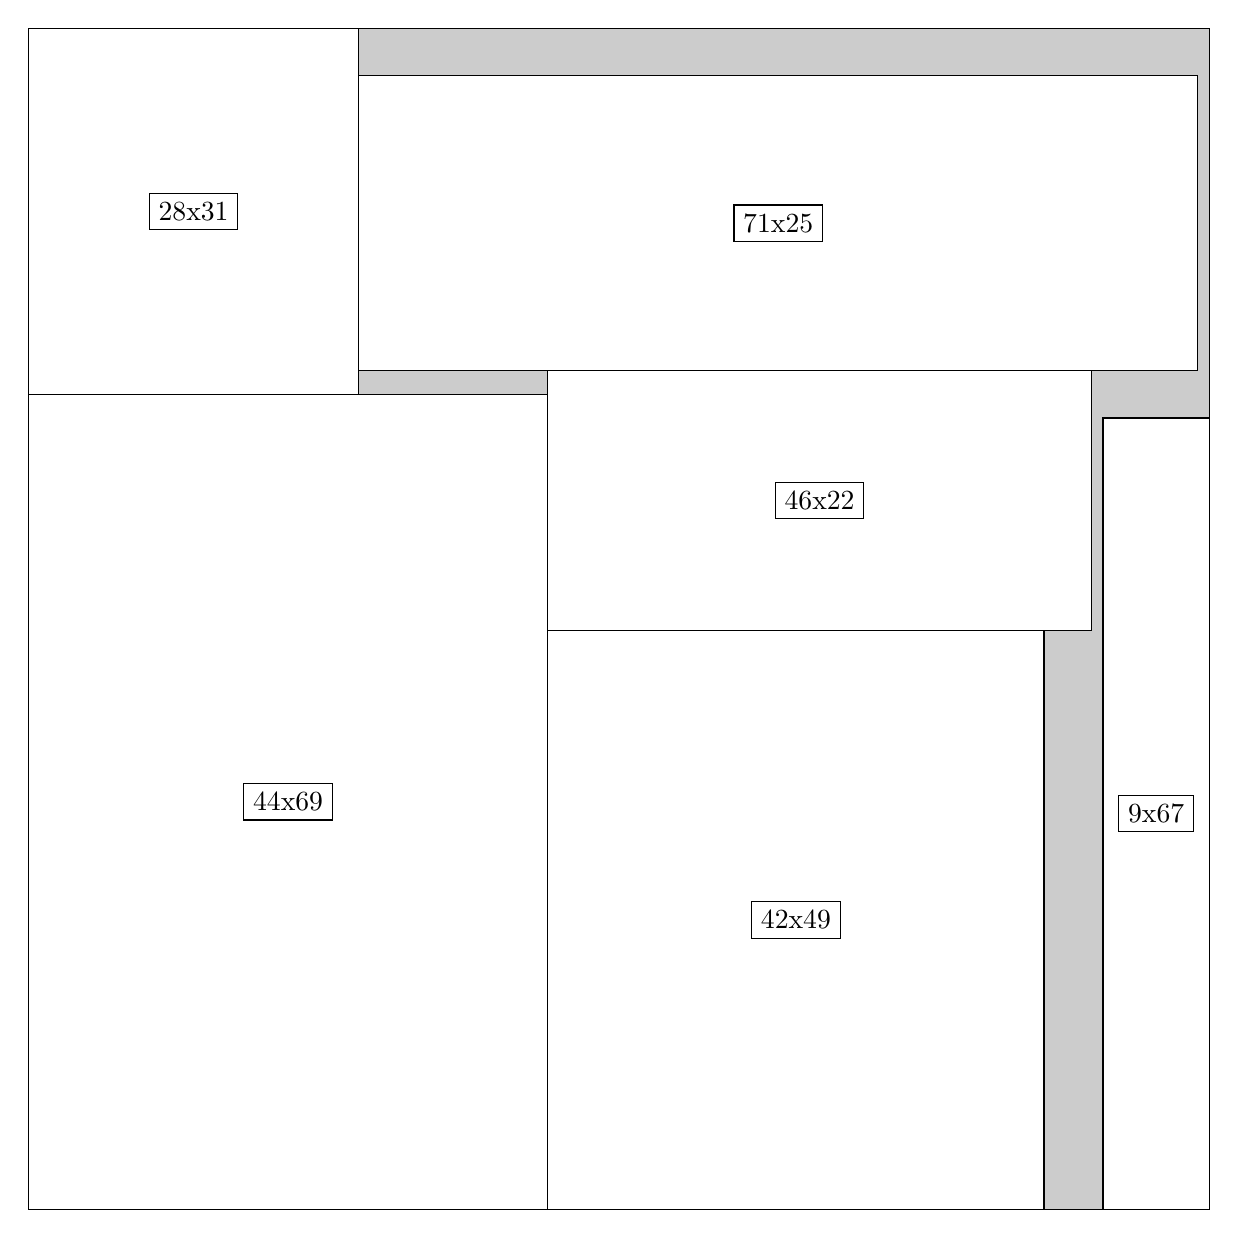
\begin{tikzpicture}[shorten >=1pt,scale=1.0,every node/.style={scale=1.0},->]
\tikzstyle{vertex}=[circle,fill=black!25,minimum size=14pt,inner sep=0pt]
\filldraw[fill=gray!40!white, draw=black] (0,0) rectangle (15.0,15.0);
\foreach \name/\x/\y/\w/\h in {44x69/0.0/0.0/6.6/10.35,42x49/6.6/0.0/6.3/7.35,71x25/4.2/10.65/10.65/3.75,46x22/6.6/7.35/6.8999999999999995/3.3,28x31/0.0/10.35/4.2/4.6499999999999995,9x67/13.65/0.0/1.3499999999999999/10.049999999999999}
\filldraw[fill=white!40!white, draw=black] (\x,\y) rectangle node[draw] (\name) {\name} ++(\w,\h);
\end{tikzpicture}


w =44 , h =69 , x =0 , y =0 , v =3036
\par
w =42 , h =49 , x =44 , y =0 , v =2058
\par
w =71 , h =25 , x =28 , y =71 , v =1775
\par
w =46 , h =22 , x =44 , y =49 , v =1012
\par
w =28 , h =31 , x =0 , y =69 , v =868
\par
w =9 , h =67 , x =91 , y =0 , v =603
\par
\newpage


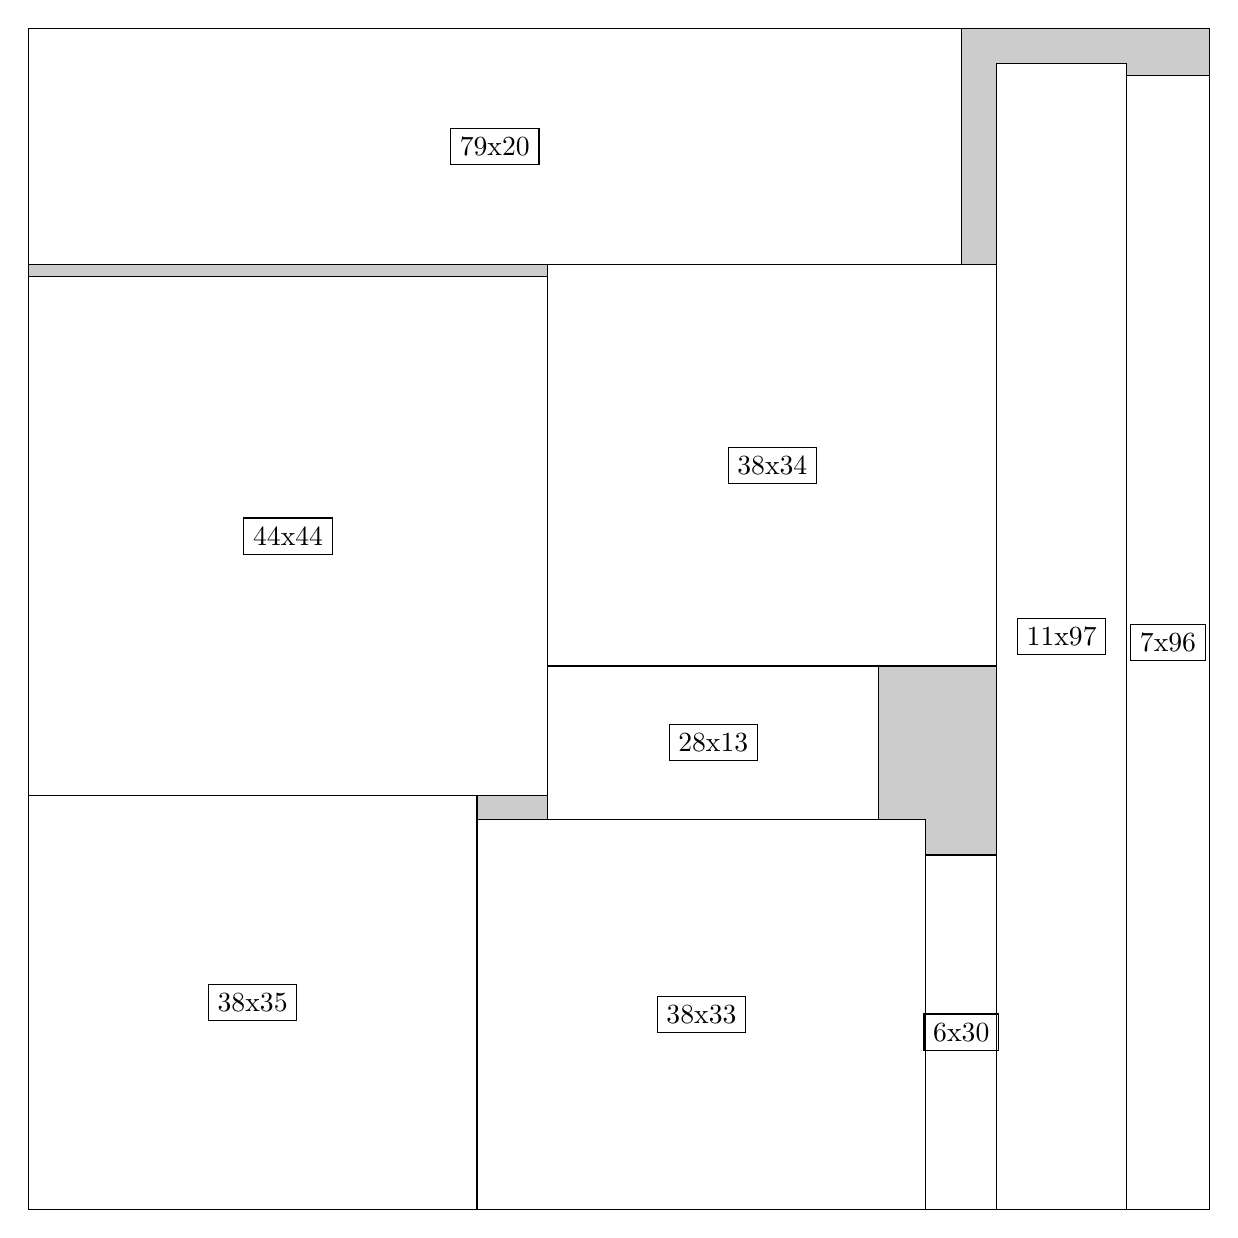
\begin{tikzpicture}[shorten >=1pt,scale=1.0,every node/.style={scale=1.0},->]
\tikzstyle{vertex}=[circle,fill=black!25,minimum size=14pt,inner sep=0pt]
\filldraw[fill=gray!40!white, draw=black] (0,0) rectangle (15.0,15.0);
\foreach \name/\x/\y/\w/\h in {38x35/0.0/0.0/5.7/5.25,44x44/0.0/5.25/6.6/6.6,79x20/0.0/12.0/11.85/3.0,38x34/6.6/6.8999999999999995/5.7/5.1,38x33/5.7/0.0/5.7/4.95,11x97/12.299999999999999/0.0/1.65/14.549999999999999,7x96/13.95/0.0/1.05/14.399999999999999,28x13/6.6/4.95/4.2/1.95,6x30/11.4/0.0/0.8999999999999999/4.5}
\filldraw[fill=white!40!white, draw=black] (\x,\y) rectangle node[draw] (\name) {\name} ++(\w,\h);
\end{tikzpicture}


w =38 , h =35 , x =0 , y =0 , v =1330
\par
w =44 , h =44 , x =0 , y =35 , v =1936
\par
w =79 , h =20 , x =0 , y =80 , v =1580
\par
w =38 , h =34 , x =44 , y =46 , v =1292
\par
w =38 , h =33 , x =38 , y =0 , v =1254
\par
w =11 , h =97 , x =82 , y =0 , v =1067
\par
w =7 , h =96 , x =93 , y =0 , v =672
\par
w =28 , h =13 , x =44 , y =33 , v =364
\par
w =6 , h =30 , x =76 , y =0 , v =180
\par
\newpage


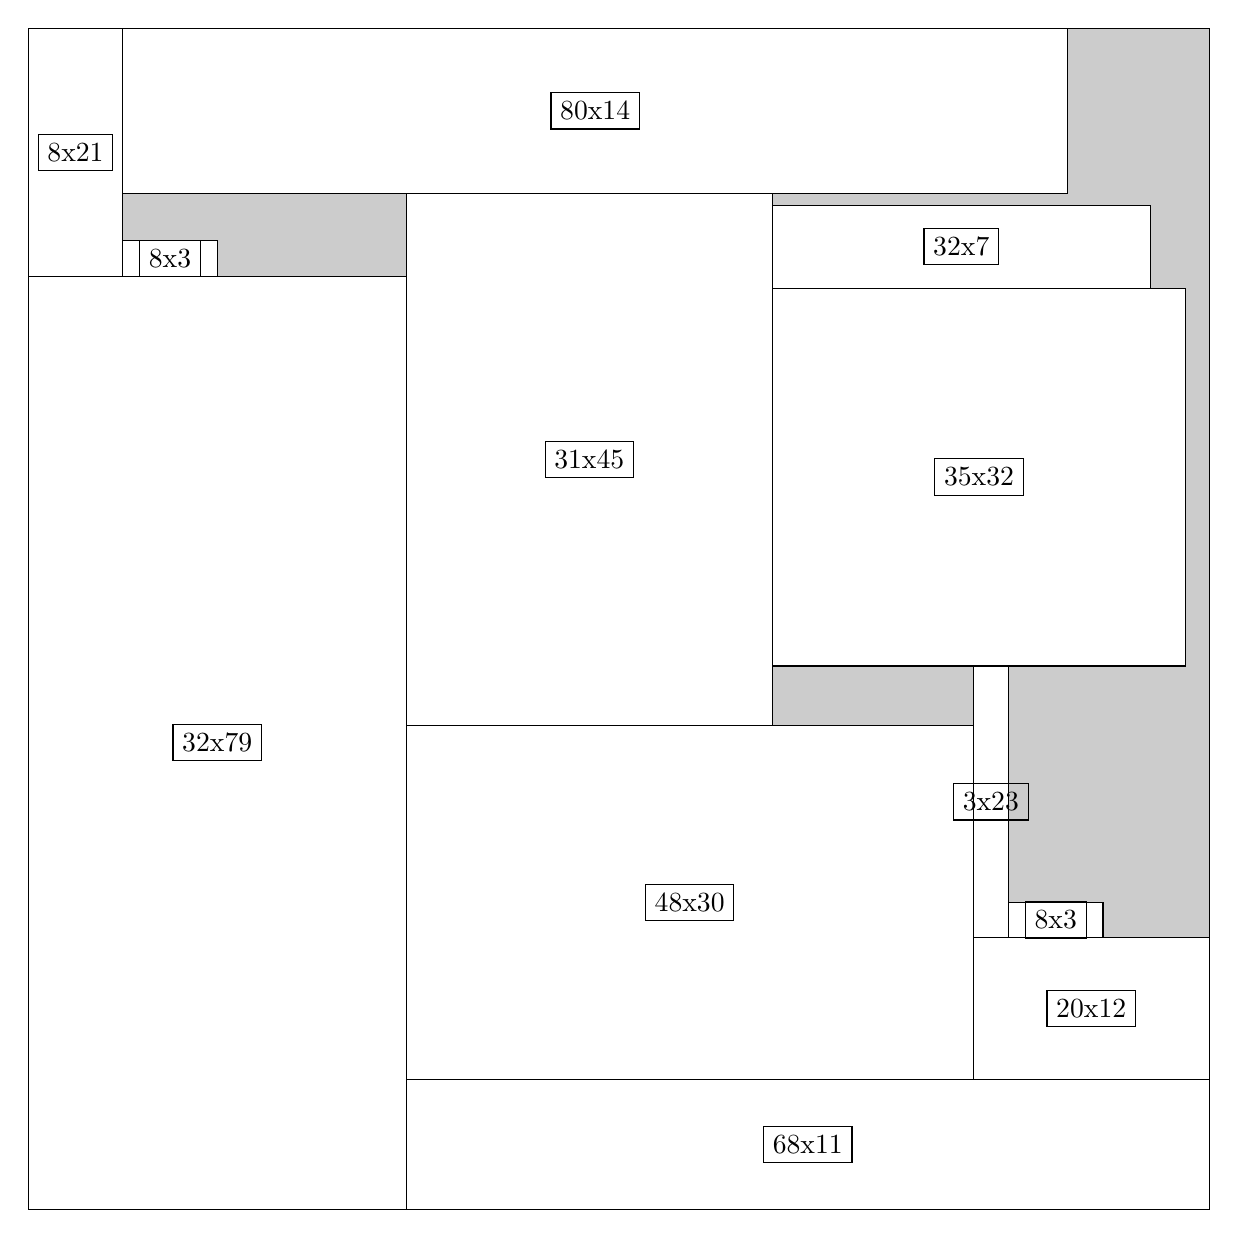
\begin{tikzpicture}[shorten >=1pt,scale=1.0,every node/.style={scale=1.0},->]
\tikzstyle{vertex}=[circle,fill=black!25,minimum size=14pt,inner sep=0pt]
\filldraw[fill=gray!40!white, draw=black] (0,0) rectangle (15.0,15.0);
\foreach \name/\x/\y/\w/\h in {32x79/0.0/0.0/4.8/11.85,48x30/4.8/1.65/7.199999999999999/4.5,31x45/4.8/6.1499999999999995/4.6499999999999995/6.75,35x32/9.45/6.8999999999999995/5.25/4.8,8x21/0.0/11.85/1.2/3.15,68x11/4.8/0.0/10.2/1.65,20x12/12.0/1.65/3.0/1.7999999999999998,32x7/9.45/11.7/4.8/1.05,80x14/1.2/12.9/12.0/2.1,3x23/12.0/3.4499999999999997/0.44999999999999996/3.4499999999999997,8x3/12.45/3.4499999999999997/1.2/0.44999999999999996,8x3/1.2/11.85/1.2/0.44999999999999996}
\filldraw[fill=white!40!white, draw=black] (\x,\y) rectangle node[draw] (\name) {\name} ++(\w,\h);
\end{tikzpicture}


w =32 , h =79 , x =0 , y =0 , v =2528
\par
w =48 , h =30 , x =32 , y =11 , v =1440
\par
w =31 , h =45 , x =32 , y =41 , v =1395
\par
w =35 , h =32 , x =63 , y =46 , v =1120
\par
w =8 , h =21 , x =0 , y =79 , v =168
\par
w =68 , h =11 , x =32 , y =0 , v =748
\par
w =20 , h =12 , x =80 , y =11 , v =240
\par
w =32 , h =7 , x =63 , y =78 , v =224
\par
w =80 , h =14 , x =8 , y =86 , v =1120
\par
w =3 , h =23 , x =80 , y =23 , v =69
\par
w =8 , h =3 , x =83 , y =23 , v =24
\par
w =8 , h =3 , x =8 , y =79 , v =24
\par
\newpage


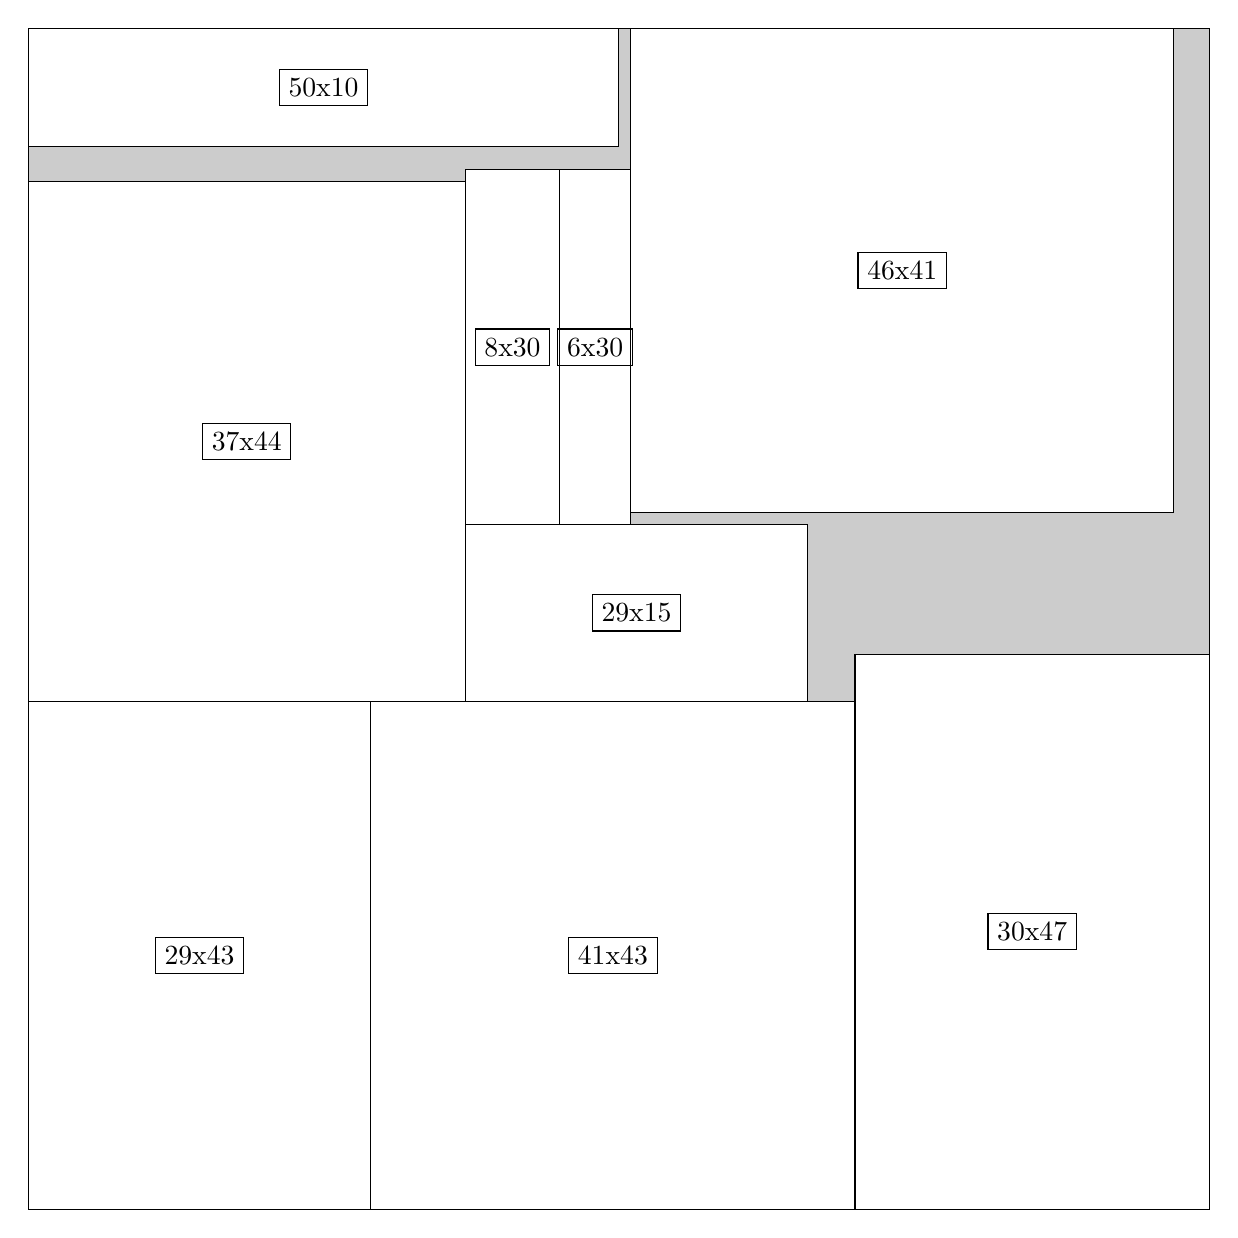
\begin{tikzpicture}[shorten >=1pt,scale=1.0,every node/.style={scale=1.0},->]
\tikzstyle{vertex}=[circle,fill=black!25,minimum size=14pt,inner sep=0pt]
\filldraw[fill=gray!40!white, draw=black] (0,0) rectangle (15.0,15.0);
\foreach \name/\x/\y/\w/\h in {29x43/0.0/0.0/4.35/6.45,41x43/4.35/0.0/6.1499999999999995/6.45,37x44/0.0/6.45/5.55/6.6,30x47/10.5/0.0/4.5/7.05,46x41/7.6499999999999995/8.85/6.8999999999999995/6.1499999999999995,50x10/0.0/13.5/7.5/1.5,29x15/5.55/6.45/4.35/2.25,8x30/5.55/8.7/1.2/4.5,6x30/6.75/8.7/0.8999999999999999/4.5}
\filldraw[fill=white!40!white, draw=black] (\x,\y) rectangle node[draw] (\name) {\name} ++(\w,\h);
\end{tikzpicture}


w =29 , h =43 , x =0 , y =0 , v =1247
\par
w =41 , h =43 , x =29 , y =0 , v =1763
\par
w =37 , h =44 , x =0 , y =43 , v =1628
\par
w =30 , h =47 , x =70 , y =0 , v =1410
\par
w =46 , h =41 , x =51 , y =59 , v =1886
\par
w =50 , h =10 , x =0 , y =90 , v =500
\par
w =29 , h =15 , x =37 , y =43 , v =435
\par
w =8 , h =30 , x =37 , y =58 , v =240
\par
w =6 , h =30 , x =45 , y =58 , v =180
\par
\newpage


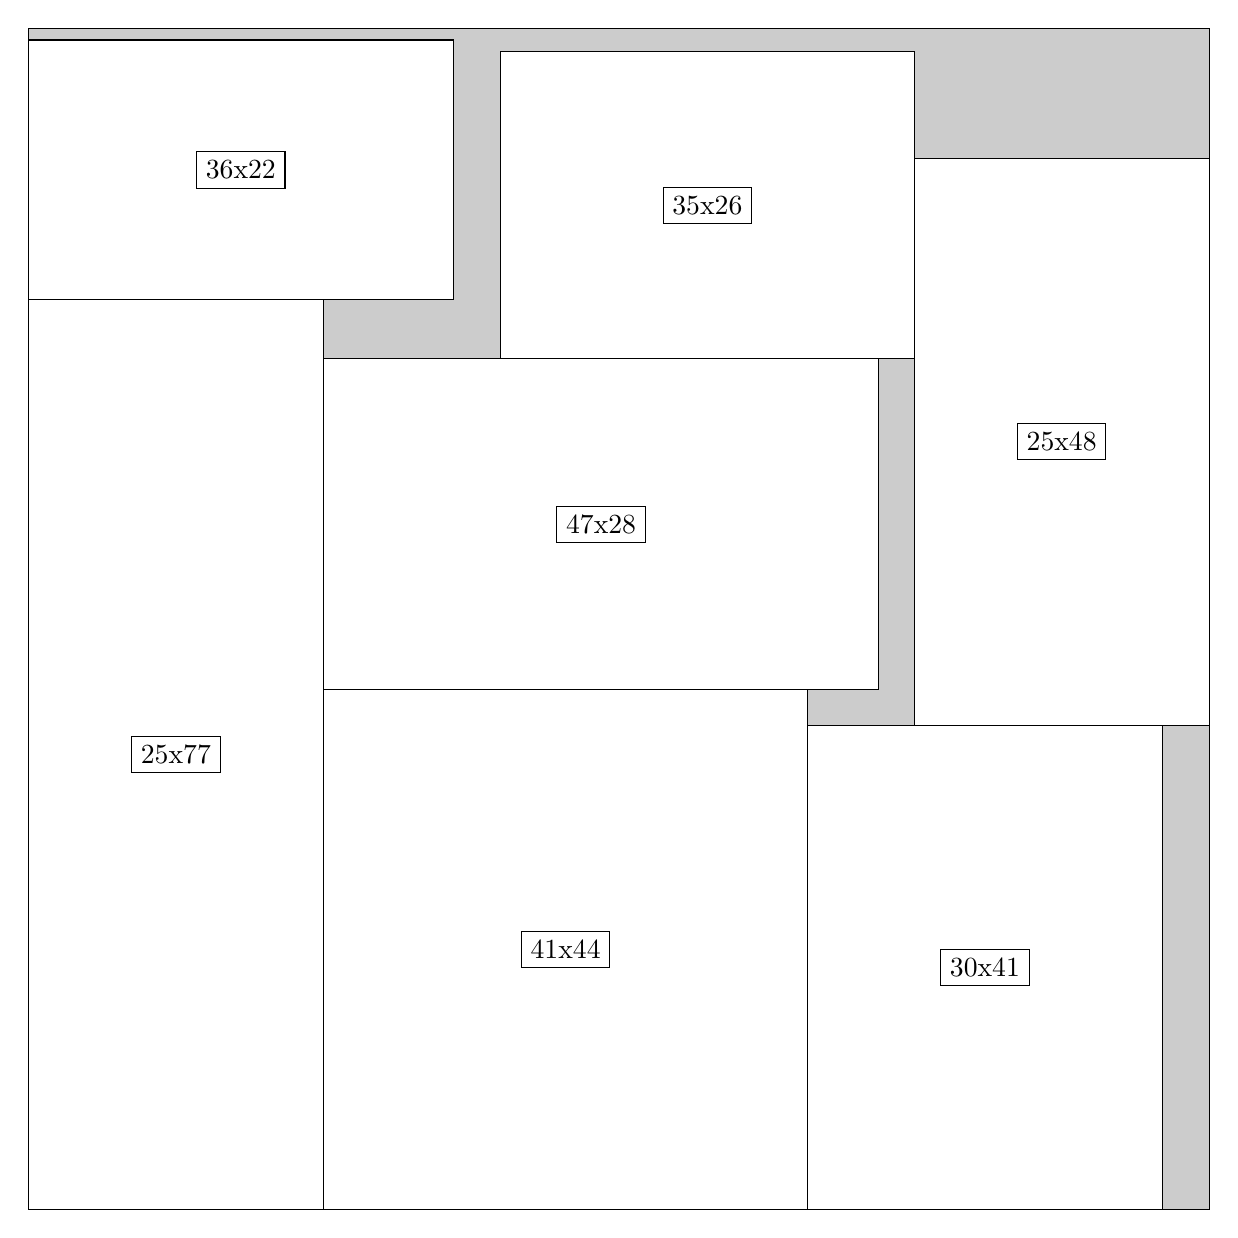
\begin{tikzpicture}[shorten >=1pt,scale=1.0,every node/.style={scale=1.0},->]
\tikzstyle{vertex}=[circle,fill=black!25,minimum size=14pt,inner sep=0pt]
\filldraw[fill=gray!40!white, draw=black] (0,0) rectangle (15.0,15.0);
\foreach \name/\x/\y/\w/\h in {25x77/0.0/0.0/3.75/11.549999999999999,41x44/3.75/0.0/6.1499999999999995/6.6,47x28/3.75/6.6/7.05/4.2,30x41/9.9/0.0/4.5/6.1499999999999995,25x48/11.25/6.1499999999999995/3.75/7.199999999999999,35x26/6.0/10.799999999999999/5.25/3.9,36x22/0.0/11.549999999999999/5.3999999999999995/3.3}
\filldraw[fill=white!40!white, draw=black] (\x,\y) rectangle node[draw] (\name) {\name} ++(\w,\h);
\end{tikzpicture}


w =25 , h =77 , x =0 , y =0 , v =1925
\par
w =41 , h =44 , x =25 , y =0 , v =1804
\par
w =47 , h =28 , x =25 , y =44 , v =1316
\par
w =30 , h =41 , x =66 , y =0 , v =1230
\par
w =25 , h =48 , x =75 , y =41 , v =1200
\par
w =35 , h =26 , x =40 , y =72 , v =910
\par
w =36 , h =22 , x =0 , y =77 , v =792
\par
\newpage


\end{document}